\chapter{Dataset Analysis}\label{appendix:dataset}

We explored the distribution of domain factors in the dataset.
The results of said exploration can be found in this chapter of the appendix.

\begin{table}[tbp]
	\centering
	\begin{tabular}{@{}crrrr@{}}
		\toprule
		& \multicolumn{3}{l}{Room Number} &             \\ 
		User        & 1         & 2         & 3       & Total       \\ \midrule
		1           & 790       & 225       & 0       & 1015        \\
		2           & 550       & 550       & 0       & 1100        \\
		3           & 300       & 375       & 150     & 825         \\
		4           & 0         & 150       & 0       & 150         \\
		5           & 225       & 150       & 0       & 375         \\
		6           & 0         & 300       & 0       & 300         \\
		7           & 0         & 0         & 150     & 150         \\
		8           & 0         & 0         & 150     & 150         \\
		9           & 0         & 0         & 150     & 150         \\
		10          & 225       & 0         & 0       & 225         \\
		11          & 225       & 0         & 0       & 225         \\
		12          & 225       & 0         & 0       & 225         \\
		13          & 225       & 0         & 0       & 225         \\
		14          & 225       & 0         & 0       & 225         \\
		15          & 225       & 0         & 0       & 225         \\
		16          & 225       & 0         & 0       & 225         \\
		17          & 225       & 0         & 0       & 225         \\ \midrule
		Total       & 3665      & 1750      & 600     & 6015        \\ \bottomrule
	\end{tabular}
	\caption{Distribution of users vs. room number in the dataset. Note that not all users are recorded in all rooms and that the room distribution is usually unbalanced. Room 3 also has the fewest number of samples by an order of magnitude.}
\end{table}

\begin{table}[tbp]
	\centering
	\begin{tabular}{@{}crrrrrrrrrrr@{}}
		\toprule
		& \multicolumn{10}{c}{Gestures}                      & \multicolumn{1}{l}{} \\ 
		User  & 1   & 2   & 3   & 4   & 5   & 6   & 7   & 8   & 9   & 10 & Total    \\ \midrule
		1     & 130 & 130 & 130 & 130 & 130 & 130 & 65  & 65  & 65  & 40 & 1015     \\
		2     & 200 & 175 & 175 & 175 & 150 & 125 & 25  & 25  & 25  & 25 & 1100     \\
		3     & 150 & 150 & 150 & 125 & 125 & 125 & 0   & 0   & 0   & 0  & 825      \\
		4     & 25  & 25  & 25  & 25  & 25  & 25  & 0   & 0   & 0   & 0  & 150      \\
		5     & 50  & 50  & 50  & 50  & 50  & 50  & 25  & 25  & 25  & 0  & 375      \\
		6     & 50  & 50  & 50  & 50  & 50  & 50  & 0   & 0   & 0   & 0  & 300      \\
		7     & 25  & 25  & 25  & 25  & 25  & 25  & 0   & 0   & 0   & 0  & 150      \\
		8     & 25  & 25  & 25  & 25  & 25  & 25  & 0   & 0   & 0   & 0  & 150      \\
		9     & 25  & 25  & 25  & 25  & 25  & 25  & 0   & 0   & 0   & 0  & 150      \\
		10    & 25  & 25  & 25  & 25  & 25  & 25  & 25  & 25  & 25  & 0  & 225      \\
		11    & 25  & 25  & 25  & 25  & 25  & 25  & 25  & 25  & 25  & 0  & 225      \\
		12    & 25  & 25  & 25  & 25  & 25  & 25  & 25  & 25  & 25  & 0  & 225      \\
		13    & 25  & 25  & 25  & 25  & 25  & 25  & 25  & 25  & 25  & 0  & 225      \\
		14    & 25  & 25  & 25  & 25  & 25  & 25  & 25  & 25  & 25  & 0  & 225      \\
		15    & 25  & 25  & 25  & 25  & 25  & 25  & 25  & 25  & 25  & 0  & 225      \\
		16    & 25  & 25  & 25  & 25  & 25  & 25  & 25  & 25  & 25  & 0  & 225      \\
		17    & 25  & 25  & 25  & 25  & 25  & 25  & 25  & 25  & 25  & 0  & 225      \\ \midrule
		Total & 880 & 855 & 855 & 830 & 805 & 780 & 315 & 315 & 315 & 65 & 6015     \\ \bottomrule
	\end{tabular}
	\caption{Distribution of users vs. gestures performed. Note that gestures 1-6 are always balanced by user, but some users performed more than others. Gestures 7-9 are performed by only some users and gesture 10 is performed by only users 1 and 2.}
\end{table}

\begin{table}[b]
	\centering
	\begin{tabular}{@{}crrrr@{}}
		\toprule
		& \multicolumn{3}{c}{Repetitions} & \multicolumn{1}{l}{} \\ 
		Room  & 5         & 10       & 20       & Total                \\ \midrule
		1     & 2025      & 950      & 690      & 3665                 \\
		2     & 1750      & 0        & 0        & 1750                 \\
		3     & 600       & 0        & 0        & 600                  \\ \midrule
		Total & 4375      & 950      & 690      & 6015                 \\ \bottomrule
	\end{tabular}
	\caption{Distribution of rooms vs repetitions. All samples were repeated at least 5 times. Specifically, in room 1, some samples were repeated 10 and 20 times.}
\end{table}

\begin{table}[tbp]
	\centering
	\begin{tabular}{@{}crrrrrrrrr@{}}
		\toprule
		& \multicolumn{8}{c}{Torso Locations}             & \multicolumn{1}{l}{} \\ 
		User  & 1    & 2    & 3    & 4    & 5    & 6  & 7  & 8  & Total                \\ \midrule
		1     & 155  & 155  & 155  & 155  & 155  & 80 & 80 & 80 & 1015                 \\
		2     & 220  & 220  & 220  & 220  & 220  & 0  & 0  & 0  & 1100                 \\
		3     & 165  & 165  & 165  & 165  & 165  & 0  & 0  & 0  & 825                  \\
		4     & 30   & 30   & 30   & 30   & 30   & 0  & 0  & 0  & 150                  \\
		5     & 75   & 75   & 75   & 75   & 75   & 0  & 0  & 0  & 375                  \\
		6     & 60   & 60   & 60   & 60   & 60   & 0  & 0  & 0  & 300                  \\
		7     & 30   & 30   & 30   & 30   & 30   & 0  & 0  & 0  & 150                  \\
		8     & 30   & 30   & 30   & 30   & 30   & 0  & 0  & 0  & 150                  \\
		9     & 30   & 30   & 30   & 30   & 30   & 0  & 0  & 0  & 150                  \\
		10    & 45   & 45   & 45   & 45   & 45   & 0  & 0  & 0  & 225                  \\
		11    & 45   & 45   & 45   & 45   & 45   & 0  & 0  & 0  & 225                  \\
		12    & 45   & 45   & 45   & 45   & 45   & 0  & 0  & 0  & 225                  \\
		13    & 45   & 45   & 45   & 45   & 45   & 0  & 0  & 0  & 225                  \\
		14    & 45   & 45   & 45   & 45   & 45   & 0  & 0  & 0  & 225                  \\
		15    & 45   & 45   & 45   & 45   & 45   & 0  & 0  & 0  & 225                  \\
		16    & 45   & 45   & 45   & 45   & 45   & 0  & 0  & 0  & 225                  \\
		17    & 45   & 45   & 45   & 45   & 45   & 0  & 0  & 0  & 225                  \\ \midrule
		Total & 1155 & 1155 & 1155 & 1155 & 1155 & 80 & 80 & 80 & 6015                 \\ \bottomrule
	\end{tabular}
	\caption{Distribution of users vs. torso locations. Torso locations are always balanced, by only user 1 performs in torso location 6-8.}
	\label{tab:dist-torso-user}
\end{table}

\begin{table}[tbp]
	\centering
	\begin{tabular}{@{}crrrr@{}}
		\toprule
		& \multicolumn{3}{c}{Room} & \multicolumn{1}{l}{} \\
		Torso Location & 1       & 2      & 3     & Total                \\ \midrule
		1              & 685     & 350    & 120   & 1155                 \\
		2              & 685     & 350    & 120   & 1155                 \\
		3              & 685     & 350    & 120   & 1155                 \\
		4              & 685     & 350    & 120   & 1155                 \\
		5              & 685     & 350    & 120   & 1155                 \\
		6              & 80      & 0      & 0     & 80                   \\
		7              & 80      & 0      & 0     & 80                   \\
		8              & 80      & 0      & 0     & 80                   \\ \midrule
		Total          & 3665    & 1750   & 600   & 6015                 \\ \bottomrule
	\end{tabular}
	\caption{Distribution of rooms vs. torso locations. Torso locations are always balanced, but torso locations 6-8 are only performed in room 1. Given that only user 1 performs these locations and the number of samples recorded by user one in Table \ref{tab:dist-torso-user} is the same as in this table, we can assume only user 1 performed in these locations.}
\end{table}

\begin{table}[tbp]
	\centering
	\begin{tabular}{@{}crrrrrr@{}}
		\toprule
		& \multicolumn{5}{c}{Face Orientation}                                     &               \\
		Room, User & 1            & 2            & 3            & 4            & 5            & Total         \\ \midrule
		\textbf{Room 1} & \textbf{733} & \textbf{733} & \textbf{733} & \textbf{733} & \textbf{733} & \textbf{3665} \\ \midrule
		1          & 158          & 158          & 158          & 158          & 158          & 790           \\
		2          & 110          & 110          & 110          & 110          & 110          & 550           \\
		3          & 60           & 60           & 60           & 60           & 60           & 300           \\
		5          & 45           & 45           & 45           & 45           & 45           & 225           \\
		10         & 45           & 45           & 45           & 45           & 45           & 225           \\
		11         & 45           & 45           & 45           & 45           & 45           & 225           \\
		12         & 45           & 45           & 45           & 45           & 45           & 225           \\
		13         & 45           & 45           & 45           & 45           & 45           & 225           \\
		14         & 45           & 45           & 45           & 45           & 45           & 225           \\
		15         & 45           & 45           & 45           & 45           & 45           & 225           \\
		16         & 45           & 45           & 45           & 45           & 45           & 225           \\
		17         & 45           & 45           & 45           & 45           & 45           & 225           \\ \midrule
		\textbf{Room 2} & \textbf{350} & \textbf{350} & \textbf{350} & \textbf{350} & \textbf{350} & \textbf{1750} \\ \midrule
		1          & 45           & 45           & 45           & 45           & 45           & 225           \\
		2          & 110          & 110          & 110          & 110          & 110          & 550           \\
		3          & 75           & 75           & 75           & 75           & 75           & 375           \\
		4          & 30           & 30           & 30           & 30           & 30           & 150           \\
		5          & 30           & 30           & 30           & 30           & 30           & 150           \\
		6          & 60           & 60           & 60           & 60           & 60           & 300           \\ \midrule
		\textbf{Room 3} & \textbf{120} & \textbf{120} & \textbf{120} & \textbf{120} & \textbf{120} & \textbf{600}  \\ \midrule
		3          & 30           & 30           & 30           & 30           & 30           & 150           \\
		7          & 30           & 30           & 30           & 30           & 30           & 150           \\
		8          & 30           & 30           & 30           & 30           & 30           & 150           \\
		9          & 30           & 30           & 30           & 30           & 30           & 150           \\ \midrule
		Total      & 1203         & 1203         & 1203         & 1203         & 1203         & 6015          \\ \bottomrule
	\end{tabular}
	\caption{Distribution of Face orientation by room and user. Face orientations are always balanced by both user and room and all face orientations are always performed, although the total number of performances by user may be different.}
\end{table}

\begin{table}[tbp]
	\centering
	\begin{tabular}{@{}crrrr@{}}
		\toprule
		& \multicolumn{3}{c}{Repetitions} & \multicolumn{1}{l}{} \\ \midrule
		Gesture & 5         & 10       & 20       & Total                \\
		1       & 650       & 115      & 115      & 880                  \\
		2       & 625       & 115      & 115      & 855                  \\
		3       & 625       & 115      & 115      & 855                  \\
		4       & 600       & 115      & 115      & 830                  \\
		5       & 575       & 115      & 115      & 805                  \\
		6       & 550       & 115      & 115      & 780                  \\
		7       & 250       & 65       &          & 315                  \\
		8       & 250       & 65       &          & 315                  \\
		9       & 250       & 65       &          & 315                  \\
		10      &           & 65       &          & 65                   \\ \midrule
		Total   & 4375      & 950      & 690      & 6015                 \\ \bottomrule
	\end{tabular}
	\caption{Distribution of repetitions vs. gestures. No specific gesture was repeated more often, but only gestures 1-6 were repeated 20 times. Gesture 10 specifically also only had 10 repetitions.}
\end{table}

\begin{figure}
	\centering
	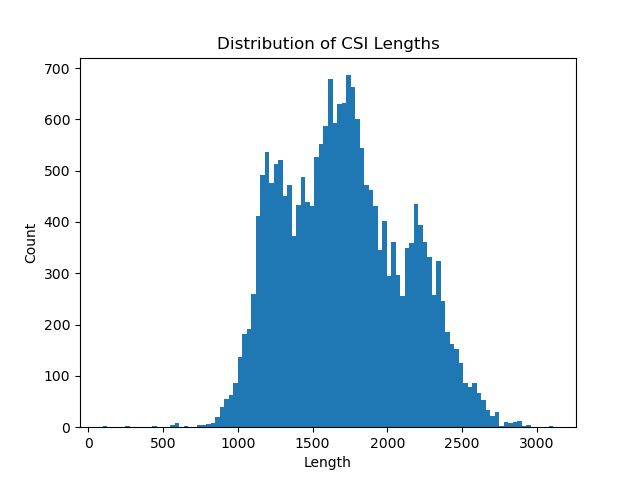
\includegraphics[width=0.7\textwidth]{figures/csi_length_distribution}
	\caption{Histogram of the length of CSI datapoints. CSI datapoints collected were of different lengths with the majority being less than 2000 samples long, representing samples of around 2 seconds each.}
\end{figure}